\usepackage{amsmath}
\usepackage{amsfonts}
\usepackage{amssymb}
\usepackage{esvect}
\usepackage{graphicx}
\usepackage{float}


\usepackage[a4paper]{geometry}
\newgeometry{left=2.5cm, right=2.5cm, bmargin=3.5cm}

\usepackage{enumitem}
\setlist{topsep=0pt, itemsep=0pt}

\parindent 0pt
\parskip 8pt
%\setlist[itemize]{noitemsep, topsep=0pt}
%\usepackage{multicol}

\usepackage{csquotes}
\usepackage{hyperref}
\title{Simulating the phototaxis response in C. Elegans}
\author{Clemens Hutter \\ chutter [at] uos.de}


%\setlist[itemize]{noitemsep, topsep=0pt}

\begin{document}



\maketitle
\begin{abstract}
The nematode C. elegans will move back once light is shown on its head. This behaviour know as phototaxis was quantified by Ward et al. \cite{Ward2008}. They looked at the timing (onset and duration) of the backward movement after light stimuli of different intensity and wavelength are applied to the worm. With the final goal to replicate the timings for all nine different stimulus configurations tested in the paper I started out with the arbitrary specific case of 350 nm and an intensity of $-1.73 \cdot log(\frac{I}{I_O})$. 
In this case the backwards movement starts roughly 1.7 seconds after stimulus onset and will last for about 7 seconds \cite{Ward2008}.
\end{abstract}

\section{Methodology} % (fold)
\label{sec:methodolegy}
I simulated the activity after the stimulus in a simplified neural network \cite{Appiah} based on the C. elegans connectome and used an evolutionary algorithm to arrive at parameters that replicate the response timing in two target motor neurons. The full source code is available here: https://github.com/rauwuckl/CElegansPhototaxis

\subsection{Network} % (fold)
\label{sub:network}
	\begin{figure}
	\centering
	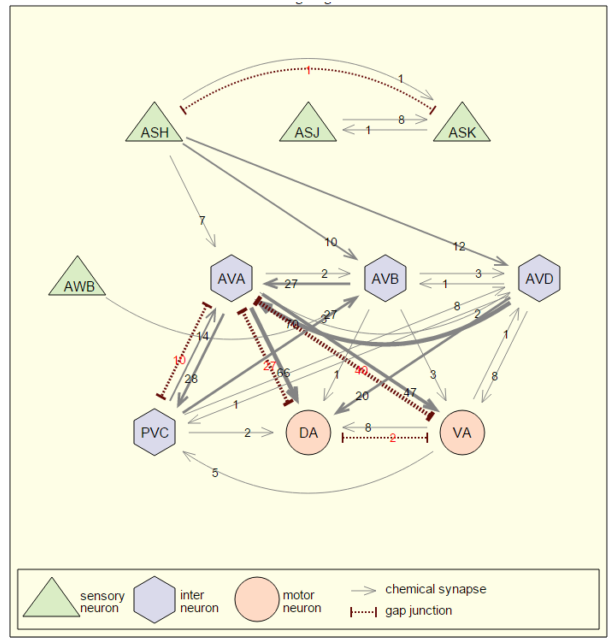
\includegraphics[width=0.5\linewidth]{network}
	\caption{Full inter neural connectivity for the sensory, interneuron and muscle neurons used in our phototaxis model.
	IV.}
	\label{fig:network}
	\end{figure}

The network (Figure \ref{fig:network}) consists of 4 sensory neurons, 4 interneurons and 2 motor neurons \cite{Appiah}. All of the neurons are modelled as Izhikevich quadratic integrate-and-fire spiking neural models \cite{izi}. (with a = 0.02, b= 0.2, c= -65, d= 6). Additionally the 4 sensory neurons receive an additive input current related to surrounding light as 
\[I_{light} = \frac{|750- \lambda| \cdot (30+i)}{\lambda}\]
where $\lambda$ is the wavelength of light (in this case 350 nm) and $i$ is the intensity (here $10^{-1.73} \cdot 20 = 0.37$) \cite{Appiah}.

Chemical synapses are modelled as Instantaneous Rise and Single-Exponential Decay synapses:
\begin{align*}
	\frac{dg}{dt} &= -\frac{1}{\tau}\cdot g  \\
	I_{syn} &= w \cdot g \cdot (V_{reversal} - V_{post})
\end{align*}
where g is the exponentially decaying conductivity which is set to 1 at each arriving presynaptic spike, $\tau$ is a time constant fixed for all synapses, $w$ is a synaptic strength constant (different value for each synapse), $V_{reversal}$ is the reversal potential ( $-70 mV$ for inhibitory and $0 mV$ for excitatory synapses), $V_{post}$ is the current membrane potential in the postsynaptic neuron and $I_{syn}$ the synaptic current that will be added to the postsynaptic neuron ($g(t) = w \cdot e ^ {-(t-t_0)/\tau} $ is an equivalent formulation). If there are connections between 2 neurons going back and forth (eg. ASJ$\rightarrow$ASK and ASK$\rightarrow$ASJ) they are explicitly modelled as 2 synapses.  

Electrical synapses are modelled symmetrical as 
\[I_{syn} = w \cdot(V_{pre} - V_{post})\]
where $w$ is again the strength for a given synapse and $V_{pre}/V_{post}$ the membrane potential in the presynaptic/postsynaptic neuron. 

There are 27 chemical and 5 electrical connections (see arrows in Figure \ref{fig:network}). Each of these connections is formed by different numbers of actual synapses (see numbers in the Figure \ref{fig:network}). Since we are assuming a global value for $\tau$ we can (for a given connection between two neurons) just add up all the synaptic currents into one combined synaptic model. The strength of theses `virtual' synapses (simply synapse from now on) will then be proportional to the number of actual synapses (numbers in Figure \ref{fig:network}). i.e. we have only one `virtual' synapse instead of 12 actual synapses from ASH to AVD but the $w$ for this synapse will be 12 times stronger. \\
Therefore our parameter space consists of 32 synaptic weights plus $\tau$. These are represented in a 33-dimensional vector $\vec{w}$ with all elements between 0 and 1. Each value of the parametervector is then mapped into a reasonable range for the corresponding  parameter:
\begin{align*}
	w^{syn}_i &= | \vec{w}_i - 0.5 |  \cdot N^{synapses}_i \cdot 0.5\\ 
	w^{electrical}_j &= (\vec{w}_j \cdot N^{synapses}_j) \in [0;1] \\
	\tau &= \vec{w}_{33} \cdot 19 + 0.1 
\end{align*}
Chemical synapses are set to excitatory for $\vec{w}_i \geq 0.5$ and inhibitory otherwise. Weights for electrical synapses are clipped such that they do not exceed [0:1]. 

The network is implemented for the brian2 simulator in Python.

% subsection network (end)

\subsection{Parameter finding with evolutionary algorithms} % (fold)
\label{sub:parmeter_finding_with_evolutionary_algorithms}
I was looking for spike patterns in the motor neurons DA and VA that could plausibly cause backwards movement starting 1.7 seconds after stimulus onset and lasting for 7 seconds \cite{Ward2008}. I argue that this would require them to start spiking before the start of the actual movement and to spike for approximately the same duration as the duration of the backward movement. Furthermore the spiking should be regular. The fitness function derived from these constrains is:
\begin{align*}
 differenceStart &= max((FirstSpike - StartResponse),0)^2\\
 differenceEnd &= max((LastSpike - EndResponse),0)^2\\
 differenceDuration &= ((LastSpike - FirstSpike) - DurationResponse)^2\\
 variance &= \textrm{variance of interspike intervals} \\
 fitness &= - (20 \cdot differeceStart + 20 \cdot differenceEnd \\&+ 20 \cdot differenceDuration + 25 \cdot variance)
\end{align*}
where the first two terms will only be non-zero if the spiking occurs after the response. The fitness is assessed for DA and VA independently in this way and then summed. 

This fitness function is optimized by the following evolutionary algorithm (adapted from \cite{Luke2013Metaheuristics}):

\begin{figure}[H]
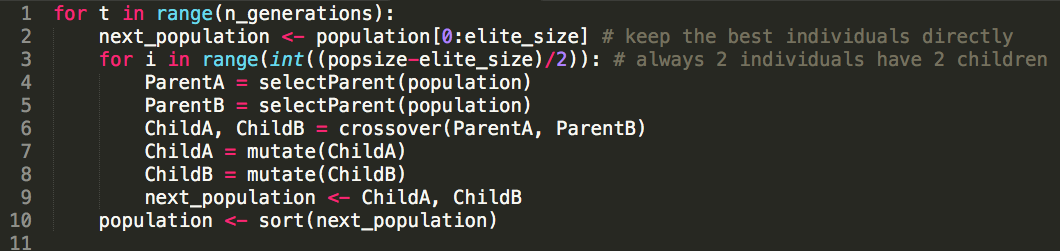
\includegraphics[width=\linewidth]{evolution}
\caption{Pseudocode for the evolutionary algorithm}
\end{figure}

\textbf{selectParent} draws 2 random individuals from the population with replacement and selects the fitter of the two. The \textbf{mutate} function simply adds independent Gaussian noise to each element of $\vec{w}$ ($\sigma = 0.001$). The \textbf{crossover} function performs \textit{Intermediate (Line) Recombination} to produce two children based on two based on two parents:

\begin{figure}[H]
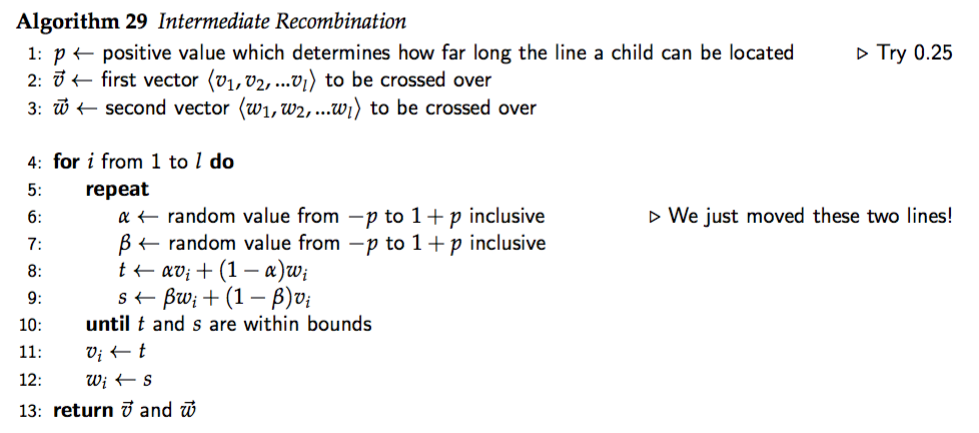
\includegraphics[width=\linewidth]{lineRecombination}
\caption{Pseudocode for Intermidiate Recombination \cite[p. 42]{Luke2013Metaheuristics}}
\end{figure}

The algorithm is implemented in Python and currently employs a multiprocess architecture to make full use of the strong PC available at the lab. To achieve this the entire population is divided into multiple subsets and the fitness in each subset is evaluated by a different job on a different CPU (Data Parallelism). For machines with only 1 or 2 cores a single threaded architecture might be faster. This can be easily changed in the source code.

% subsection subsection_name (end)'
\section{Results} % (fold)
\label{sec:results}
If no noise is added to the membrane potential of the neurons a very good fit is quite easily achievable. But real neurons will undoubtedly be subject to some noise. In this case the quality of a given parameter set $\vec{w}$ will vary considerably from run to run. So the fitness function for a given individual (parameter set) is extremely stochastic.

For this summery I left the evolution running for 82 generations, while evaluating the fitness for each individual at each generation 4 times and averaging over it to achieve a somewhat reliable value. 
Then I simulated the network for the fittest individual nine times to give a rough idea of the different activity patterns that arise. 

\begin{itemize}
	\item In the best case scenario the network very precisely replicated the response timing (Figure \ref{fig:optimalRun}). 
	\item The most common outcome however can be seen in Figure \ref{fig:noStop}. Here the network starts spiking but does not calm back down to rest within the simulation time of 10.5 seconds. 
	\item Also common is that the response will last exactly as long as the stimulus exiting the network (Figure \ref{fig:imideateStop}).
\end{itemize}


\begin{figure}[H]
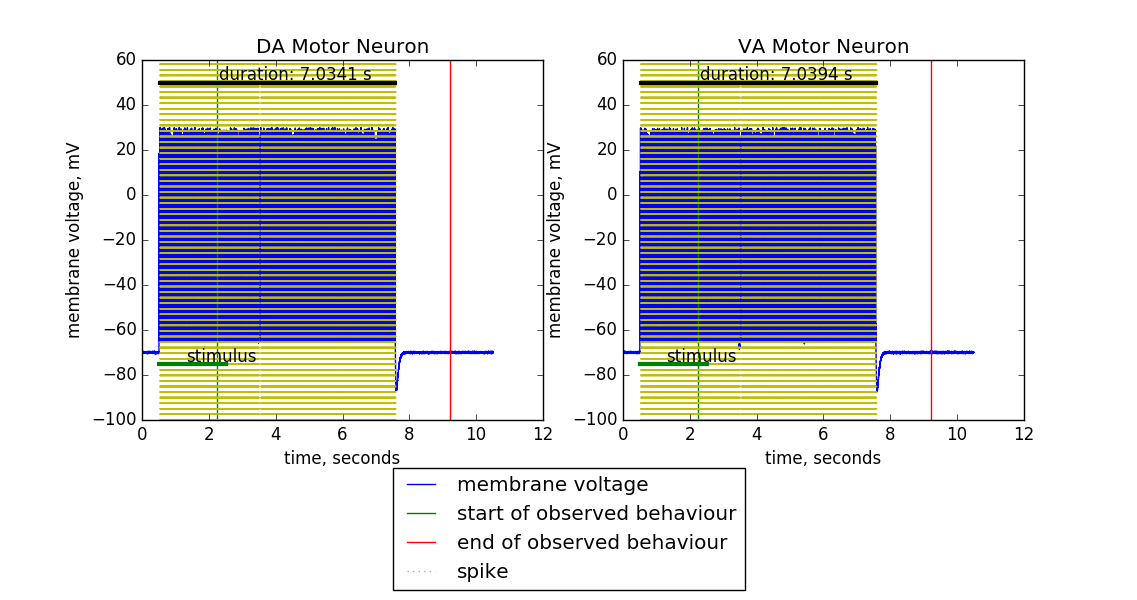
\includegraphics[width=\linewidth]{perfect}
\caption{Trace of optimal run. (3 out of 9 runs with response durations of 7.0, 7.1 and 6.0 seconds)}
\label{fig:optimalRun}
\end{figure}
\begin{figure}[H]
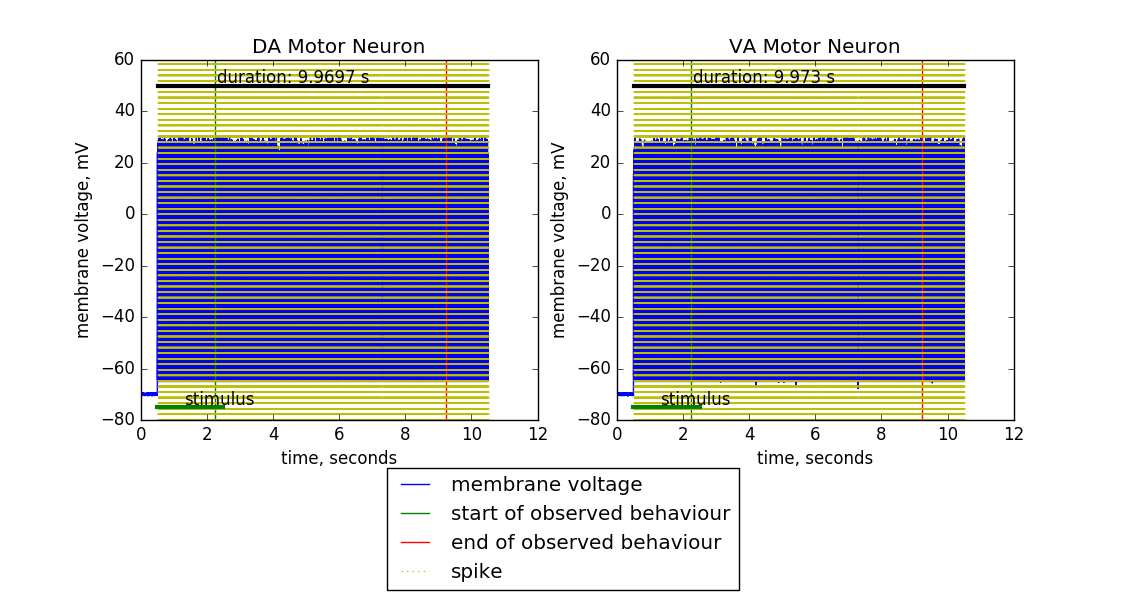
\includegraphics[width=\linewidth]{noStop}
\caption{Most common trace. Spiking does not stop. (5 out of 9 runs)}
\label{fig:noStop}
\end{figure}
\begin{figure}[H]
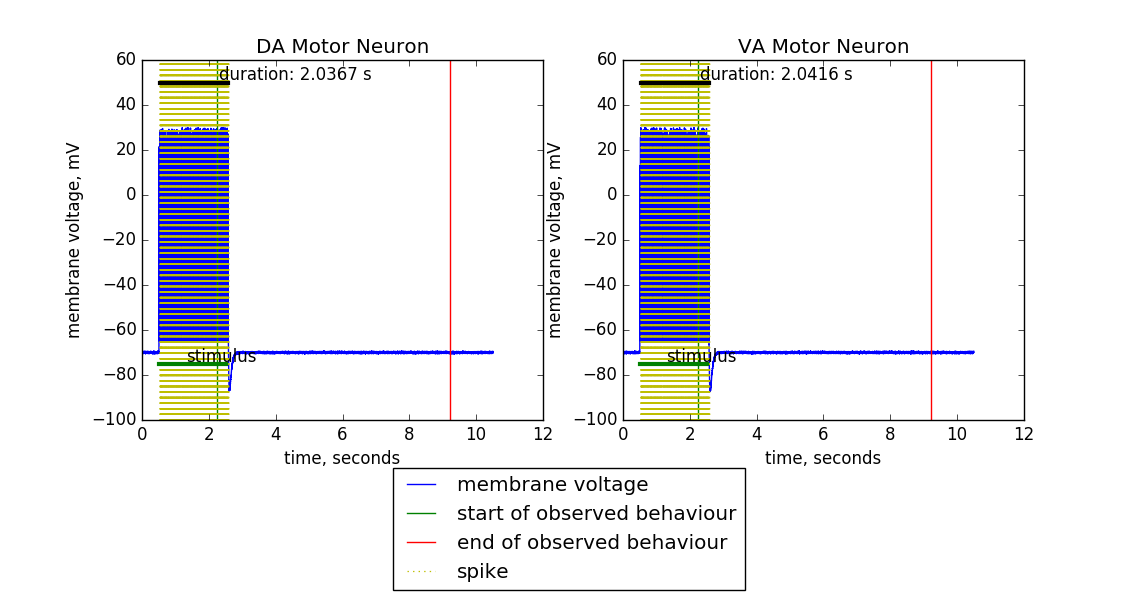
\includegraphics[width=\linewidth]{imideateStop}
\caption{Spiking stops immediately. (1 out of 9 runs)}
\label{fig:imideateStop}
\end{figure}

\section{Discussion} % (fold)
\label{sec:discussion}
I believe that the target response we are trying to achieve within the network is very unstable. The network has to get excited by external input which then is turned off after which the spiking response must not change. Then it has to stay excited for a set amount of time and after that it autonomously has to calm down without any change in input. \\
This I think happens once a short interval occurs in which all neurons in the highly recursive network are \textit{`by chance'} in their refractory period. Then the self sustaining circle of excitation is stopped and the activity fades away. But as soon as we add even a little noise the exact spike times of all neurons will be shifted a little against each other. The interval of accidental silence can now occur at a completely different time (or not at all). Because of this intuition I figure that it is impossible to find parameters which are able to reproduce the behaviour reliable over multiple runs. 

Also it is still unclear how higher activity in those two motorneurons actually relates to backward movement. 

\small{Disclaimer: \textit{What is referred to as neurons (DMA, AVA, etc.) in this paper are actually neuron classes.}}

\bibliographystyle{unsrt}%alternative alpha
\bibliography{bibliography}

\end{document}




